\chapter{Análisis y Diseño}

En las etapas iniciales de la metodología ``Cascada'', se realiza el análisis del problema y diseño previo del sistema, todo esto al inicio de la implementación del producto final. Es importante que estas fases sean completadas en su totalidad para que el desarrollo sea exitoso. Este proyecto plantea el diseñado y desarrollo para 70 dias hábiles según calendario, con la distribución del tiempo definido según la complejidad de las tareas que implican cada una de las fases.\\

\section{Análisis}
Para el diseño del Sistema de Video-Vigilancia Inteligente, es necesario tener en cuenta los elementos principales que lo componen. Un sistema de video-vigilancia esta compuesto de cámaras individuales y un puesto central o servidor donde todas las conexiones convergen y se centralizan para su control. En el dispositivo central (servidor) se procesan las imágenes que las cámaras capturan y se convierten en video para ser visualizado en un monitor.\\

El sistema propuesto permite visualizar video en vivo desde cualquier dispositivo con acceso a la red de internet además de que envía notificaciones automáticas en el instante en que se detecta: movimiento, fuego, o silueta de un intruso. El usuario recibe la notificación por correo electrónico el cual adjunta capturas y un enlace web para visualizar en vivo lo que esta captando la cámara.\\

% Los principales módulos del sistema son:
% \begin{itemize}
%     \item Módulo de cámara (Nodos)
%     \item Módulo de servidor (Analizador y noti)
%     % \item Servidor HTTP (Servicio que aplica el protocolo de la Web)
%     % \item Módulo SMTP (Módulo de envio de correo electrónico)
% \end{itemize}

En la figura \ref{fig:system_desing} se visualiza el esquema general del sistema propuesto. Las cámaras de video-vigilancia se encargan de capturar los fotogramas de video y se enlazan por medio de un socket o conector (uno por cada cámara) al servidor central. Cuando es registrada una nueva conexión, el sistema notifica al usuario por medio de un correo electrónico, compartiendo información relevante sobre la conexión de una nueva cámara. El servidor central, maneja todas las conexiones, además realiza el análisis de los fotogramas de manera individual por cada cámara conectada por medio de una libreria de visión por computadora. De forma paralela se construye el video que se va a transmitir a partir de los fotogramas, siendo decodificado por medio de un conjunto de paquetes de software libre, los cuales arman las partes del archivo para el streaming de video por medio de la red. Cuando un evento (fuego, movimiento, silueta humana) es identificado, automáticamente el sistema envia la notificación correspondiente por medio de correo electronico al usuario avisando una posible situación identificada.\\

\begin{figure}[H]
    \begin{center}
        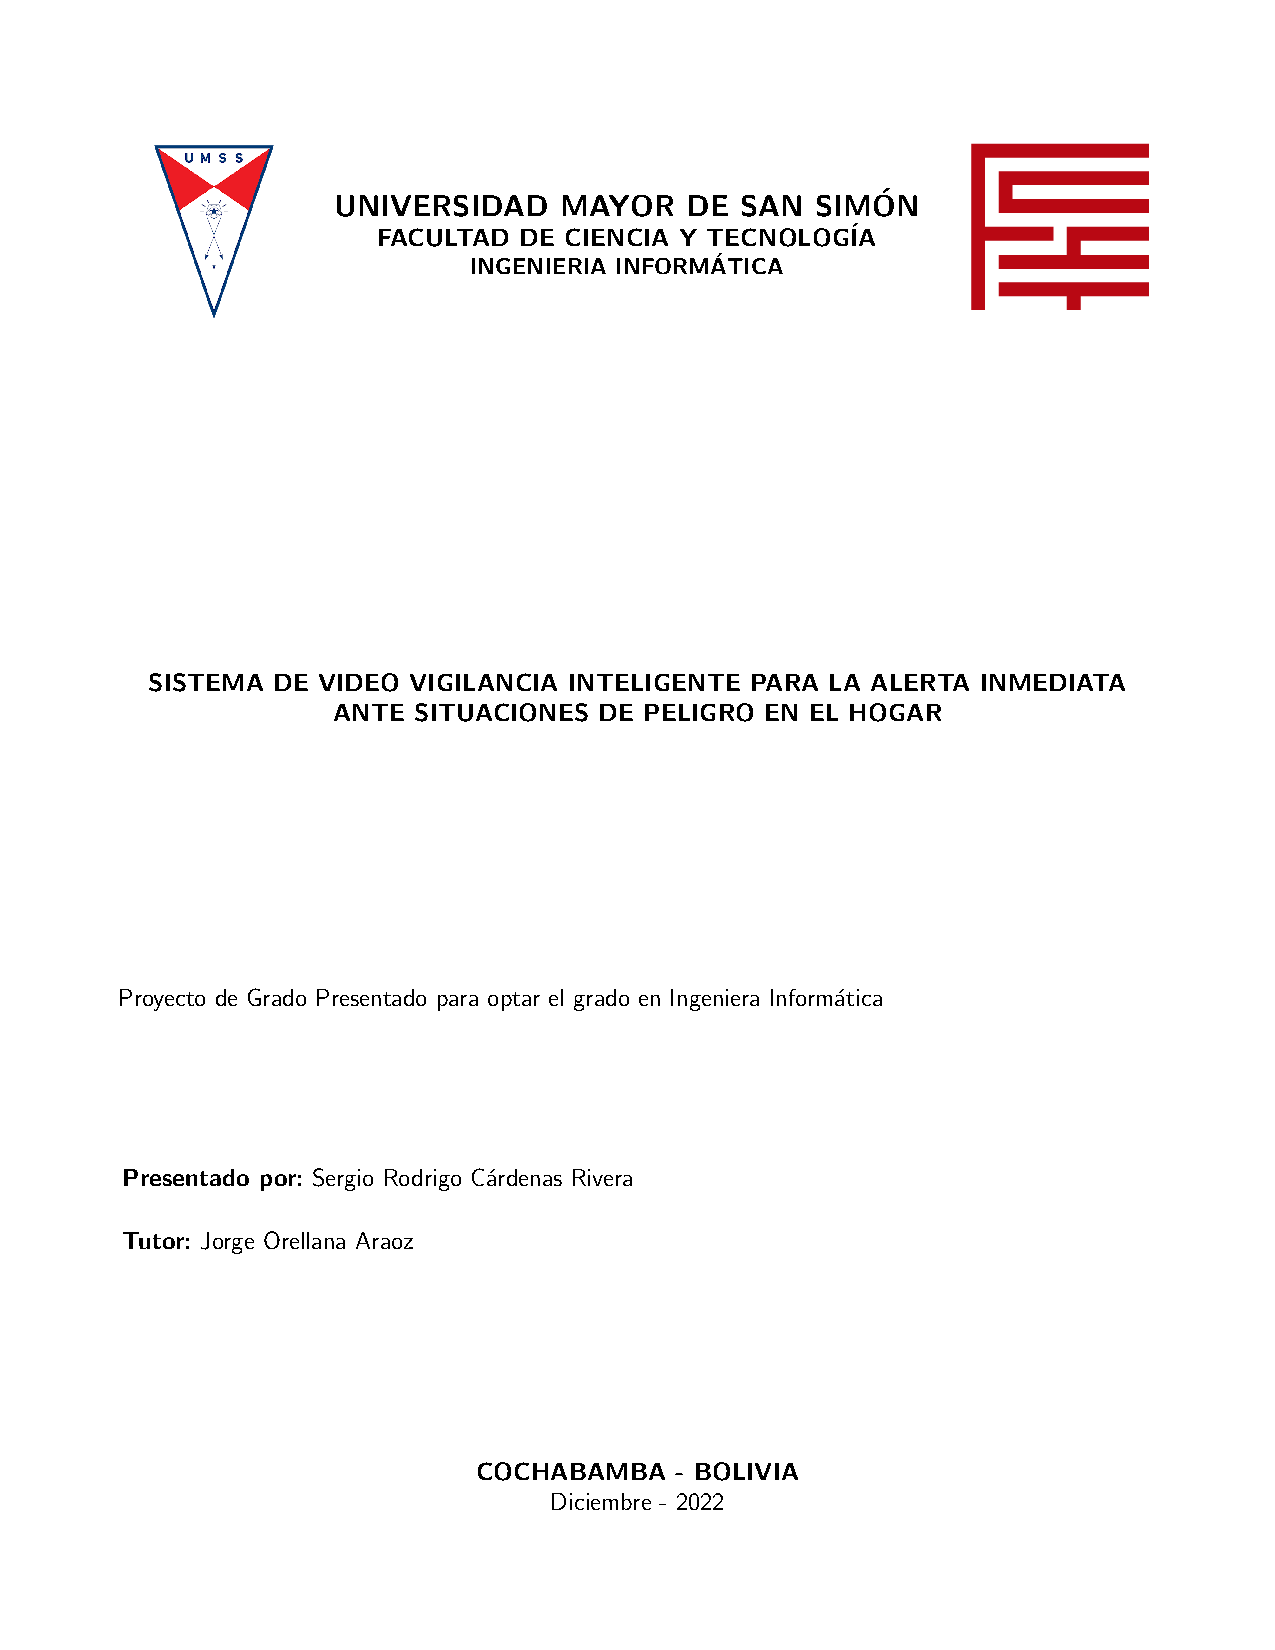
\includegraphics[width=17cm]{img/capitulo_4/main.jpeg}
        \caption{Diseño de interacción de los módulos del sistema de video-vigilancia.}
        Fuente : Elaboración propia
        \label{fig:system_desing}
    \end{center}
\end{figure}

\subsection{Definición de Requerimientos}
La definición de requerimientos es una de las actividades más importantes del desarrollo de software; de ello depende el resto de actividades del proyecto. Anteriormente se describe completamente el comportamiento del sistema que se desarrolla para la identificación de los requerimientos. Inicialmente se plantean los criterios de partida a tomar en cuenta en el diseño del sistema de video-vigilancia inteligente:

\begin{itemize}
    \item Costos altos en la infraestructura de transmisión de video en vivo.
    \item Las características de identificación automática, estan disponibles para sistemas de video-vigilancia de alto nivel.
    \item Una alerta inmediata puede minimizar el impacto de alguna situación que ponga en peligro la integridad de bienes materiales y humanos.
    \item Los usuarios finales son personas que a menudo dejan su hogar para salir a trabajar, y usan constamente su correo electrónico.
\end{itemize}

\subsubsection{Requerimientos Funcionales}
En esta fase es necesario delimitar el alcance y las capacidades del sistema planteado para la realización de la planificación inicial, estimación de tiempos, diseño y desarrollo. Para ello se define la lista de requerimientos funcionales del sistema de video-vigilancia inteligente.

\begin{table}[H]
    \caption{Lista de requerimientos funcionales }
    \label{tabla:req_funcionales}
    \begin{center}
        \begin{tabular}{ |c|l|} 
            \hline
            1. & Capturar fotogramas por medio de una o varias cámaras portatiles.\\ \hline
            2. & Visualizar fotogramas capturados en tiempo real (captura de video).\\  \hline
            3. & Notificar al usuario cuando una nueva cámara se conecta.\\  \hline
            4. & Notificar al usuario cuando una cámara se desconecta.\\  \hline
            5. & Enviar fotogramas capturados por medio de la red al servicio encargado de su análisis.\\ \hline
            6. & Análizar y procesar fotogramas capturados individualmente por cada cámara.\\  \hline
            7. & Permitir la recepción de fotogramas de varias fuentes hacia el servicio.\\ \hline
            8. & Transmitir los fotogramas convertidos en video en vivo desde fuentes diferentes.\\ \hline
            9. & Detectar movimiento a partir de fotogramas recibidos desde distintas fuentes.\\ \hline
            10. & Detectar silueta humana a partir de fotogramas recibidos desde distintas fuentes.\\ \hline
            11. & Detectar fuego a partir de fotogramas recibidos desde distintas fuentes.\\ \hline
            12. & Notificar al usuario por medio de un correo electrónico cuando se de una detección.\\ \hline
        \end{tabular}
    \end{center}
    \begin{center}
        Fuente: Elaboración propia.
    \end{center}
\end{table}

\subsubsection{Requerimientos No Funcionales}
Los requerimientos no funcionales son aquellos relacionados con la calidad y el proceso de desarrollo del sistema. Los tipos de requisitos no funcionales aplican: rendimiento, disponibilidad, accesibilidad, usabilidad, estabilidad, portabilidad, costo, operatividad, interoperabilidad, escalabilidad, concurrencia, mantenibilidad, interfaz, plazo de entrega y herramientas. Los requisitos no funcionales surgen de la necesidad del usuario, debido a las restricciones en el presupuesto y las herramientas utilizadas.\\

\begin{enumerate}
    \item  \textbf{Requisitos de interfaz} 
        \begin{itemize}
            \item Las cámaras tendran una interfaz que permita visualizar la tarea que ejecutan.
            \item El servidor mostrará información necesaria sobre las tareas que realiza.
            \item El sistema deberá ser de fácil configuración.
            \item Las notificaciones por correo electrónico deberán ser visualmente estilizadas.
        \end{itemize}
    \item \textbf{Requisitos de portabilidad}
        \begin{itemize}
            \item Los módulos de cámara podran conectarse de forma cableada o inalámbrica.
        \end{itemize}
    \item \textbf{Requisitos de disponibilidad}
        \begin{itemize}
            \item La transmisión en vivo estará disponible cuando el usuario quiera visualizar lo que captan las cámaras.
        \end{itemize}
\end{enumerate}

\section{Planificación}
Todas las fases del modelo cascada son planificadas según la complejidad y tareas que presenta cada fase. Dado que cada fase debe culminarse por completo para pasar a la siguiente o en su defecto requerir mínimas modificaciones para regresar a la fase anterior, se plantea una planificación de 70 días hábiles que se visualiza en la tabla \ref{tabla:planning}.\\

\begin{table}[H]
    \caption{Tabla de planificación según fases del modelo Cascada.}
    \label{tabla:planning}
    \begin{center}
        \begin{tabular}{|c|l|c|c|c|}
            \hline
            \textbf{Num.} & \textbf{Fase del modelo Cascada}  &  \textbf{Fecha inicial} & \textbf{Fecha final} & \textbf{Duración (días)}\\ \hline
            \textbf{1.} & Fase de análisis        & 6-jun        & 17-jun        & 10        \\ \hline
            \textbf{2.} & Fase de diseño del sistema       & 20-jun        & 8-jul        & 15        \\ \hline
            \textbf{3.} & Fase de implementación        & 11-jul        & 19-ago        & 30        \\ \hline
            \textbf{4.} & Fase de pruebas        & 22-ago         &   2-sep     &    10     \\ \hline
            \textbf{5.} & Fase de mantenimiento        & 5-sep        & 9-sep        & 5        \\ \hline
        \end{tabular}
        \begin{center}            
            Fuente: Elaboración propia.
        \end{center}
    \end{center}
\end{table}

En la figura \ref{fig:gannt} se visualiza e diagrama de Gannt en base a la planificación expresada en la anterior tabla.
\begin{figure}[H]
    \begin{center}
        \includegraphics[width=18cm]{img/capitulo_4/gant.png}
    \end{center}
    \begin{center}
        \caption{Diagrama de Gannt.}
        Fuente : Elaboración propia
        \label{fig:gannt}
    \end{center}
\end{figure}

\section{Diseño}
El diseño del sistema de video-vigilancia se divide y se desarrolla según los módulos que componen el sistema completo:
\begin{itemize}
    \item Módulo de cámaras
    \item Módulo de servidor
\end{itemize}

\subsection{Módulo de cámaras}
El módulo de cámaras permite el control de conexión de una cámara al servidor central. Permite conectar una cámara web o una cámara de  una Raspberry Pi. Presenta campos para ingresar datos de configuración que permiten la conexión al servidor central.\\

\subsubsection{Diseño de interfaz}
En la figura \ref{fig:cam_user_interface} se presenta el esbozo de interfaz de ususario que servirá de diseño final para el desarrollo del presente módulo. El módulo de cámaras permite la visualizacion de fotogramas capturados por medio de la cámara conectada, configuración de la conexión y verificación del estado de envio de los fotogramas al servidor.

\begin{figure}[H]
    \begin{center}
        \includegraphics[width=13cm]{img/capitulo_4/camera_interface.png}
    \end{center}
    \begin{center}
        \caption{Diseño de interfaz gráfica de usuario (Módulo de cámaras).}
        Fuente: Elaboración propia.
        \label{fig:cam_user_interface}
    \end{center}
\end{figure}

A continuación se describe a detalle cada uno de los elementos que conforman la interfaz de usuario del módulo de cámaras.
\begin{enumerate}
    \item \textbf{Pantalla}: Espacio de  visualización de los fotogramas que capta la cámara conectada.
    \item \textbf{Botón WebCam}: Botón de conexión/desconexión para la cámara web
    \item \textbf{Botón PiCam}: Botón de conexión/desconexión para la cámara de Raspberry Pi.
    \item \textbf{Campo de dirección IP}: Campo de texto para que el usuario ingrese la dirección IP del servidor.
    \item \textbf{Campo de número de puerto}: Campo de texto para que el usuario ingrese el puerto de escucha del servidor.
    \item \textbf{Campo de identificador de la cámara}: Campo de texto para que el usuario ingrese el número identificador de la cámara conectada.
    \item \textbf{Botón de conexión}: Botón de conexión/desconexión al servidor para el envio de fotogramas al servidor.
    \item \textbf{Cuadro de mensajes}: Cuadro de lista para mostrar diferentes mensajes de módulo: envio de fotogramas, conexión/desconexión al servidor, etc.
\end{enumerate}

\subsubsection{Diagrama de secuencia}
En la figura \ref{fig:diag_sec_mod_camera} se ilustra el diagrama de secuencia del módulo de cámaras. El diagrama describe de forma gráfica el comportamiento de la interacción entre el módulo de cámaras con el servidor.

\begin{figure}[H]
    \begin{center}
        \includegraphics[width=7cm]{img/capitulo_4/sec_cam_serv.jpg}
    \end{center}
    \begin{center}
        \caption{Diagrama de interacción entre el módulo de cámaras con el servidor.}
        Fuente: Elaboración propia.
        \label{fig:diag_sec_mod_camera}
    \end{center}
\end{figure}

La interacción entre el módulo cámaras y el servidor es como sigue:
\begin{enumerate}
    \item El módulo de cámaras realiza una petición de conexión al servidor.
    \item El servidor acepta la petición y le asigna un puerto de escucha a esa nueva conexión.
    \item Se registra el identificador de la cámara para evitar duplicidad en los identificadores.
    \item El servidor envia un mensaje de confirmación de conexión.
    \item El módulo de cámaras envia un fotograma.
    \item El servidor confirma la recepción del fotograma.
    \item Se repiten los anteriores pasos mientras dura la conexión.
    \item El módulo de cámaras se desconecta del conector asignado.
    \item El servidor elimina el registro del identificador de la cámara y libera la conexión. 
\end{enumerate}

% \subsubsection{Diagrama de estado}
% Se estudia los casos en los que el usuario interactura con el módulo de cámara.
% \begin{itemize}
%     \item Usuario inicializa la cámara
%     \item Ingresa la configuracion
%     \item Si hay un dispositivo con la misma configuracion se recahza la conexión.
%     \item sigue el proceso exitoso.
% \end{itemize}
\subsubsection{Diagrama de clases}
De acuerdo al planteamiento de comportamiento del módulo de cámaras, para el desarrollo de este módulo se plantea el diagrama de clases que se visualiza en la figura \ref{fig:camera_clases}.\\

\begin{figure}[H]
    \begin{center}
        \includegraphics[width=15cm]{img/capitulo_4/camera_clases.jpg}
        \caption{Diagrama de clases del módulo de cámaras.}
        Fuente : Elaboración propia
        \label{fig:camera_clases}
    \end{center}
\end{figure}

Para la comprensión de este diagrama de clases se procede a describir cada clase con sus respectivos atributos y métodos.\\

\begin{itemize}
    \item \textbf{Main}: Es la clase principal que se encarga de cargar todas las instancias del necesarias para el módulo de cámaras. Estos son sus atributos:
        \begin{itemize}
            \item settings: Instancia de la clase Settings, que permite cargar las configuraciones iniciales para iniciar el módulo.
            \item node: Instancia de la clase Node, que representa el ciclo de petición de los fotogramas de la cámara.
            \item connection: Instancia de la clase Connection, que permite la conexión/desconexión con el servidor a partir de la configuracion por defecto establecida en el archivo de configuración inicial.
        \end{itemize}
        Los métodos de clase son:
        \begin{itemize}
            \item run\_node: Método que se encarga de iniciar la vista de la interfaz de usuario en base a la configuración del módulo.
        \end{itemize}
    \item \textbf{Node}: Esta clase se encarga de implementar los métodos que permiten obtener los fotogramas directamente cual se la cámara conectada (WebCam o PiCam) como tambien de enviar los fotogramas tanto al servidor como a la pantalla para su visualización. Este es su único atributo:
        \begin{itemize}
            \item camera: Es la instancia de la cámara que permite la captura de fotogramas.            
        \end{itemize}
        Los métodos de clase son:
        \begin{itemize}
            \item execute: 
            \item stop\_node:
        \end{itemize}
    \item \textbf{Settings}
        Estos son sus atributos:
        \begin{itemize}
            \item Settigns :
            \item Node :
            \item Connection :
        \end{itemize}
        Estos son sus métodos
        \begin{itemize}
            \item run\_node :
        \end{itemize}
    \item \textbf{Connection}
        Estos son sus atributos:
        \begin{itemize}
            \item Settigns :
            \item Node :
            \item Connection :
        \end{itemize}
        Estos son sus métodos
        \begin{itemize}
            \item run\_node :
        \end{itemize}
    \item \textbf{Camera}
        Estos son sus atributos:
        \begin{itemize}
            \item Settigns :
            \item Node :
            \item Connection :
        \end{itemize}
        Estos son sus métodos
        \begin{itemize}
            \item run\_node :
        \end{itemize}
    \item \textbf{WebCamera}
        Estos son sus atributos:
        \begin{itemize}
            \item Settigns :
            \item Node :
            \item Connection :
        \end{itemize}
        Estos son sus métodos
        \begin{itemize}
            \item run\_node :
        \end{itemize}
    \item \textbf{PiCamera}
        Estos son sus atributos:
        \begin{itemize}
            \item Settigns :
            \item Node :
            \item Connection :
        \end{itemize}
        Estos son sus métodos
        \begin{itemize}
            \item run\_node :
        \end{itemize}
\end{itemize}

\subsection{Módulo de servidor}
El servidor que se encarga de la transmision
\subsubsection{Diagrama de secuencia}
Se describe el proceso entre el servidor y la cámara para el respectivo análisis de los frames

\begin{figure}[H]
    \begin{center}
        \includegraphics[width=12cm]{img/capitulo_4/camera_notif.png}
    \end{center}
    \begin{center}
        \caption{Diagrama de secuencia: Notificación de conexión/desconexión.}
        Fuente: Elaboración propia.
        \label{fig:diag_sec_notif_conn}
    \end{center}
\end{figure}

A continuación se describe la interacción entre la cámara, el servidor y el proceso de notificación:
\begin{enumerate}
    \item El módulo de cámaras realiza una petición de conexión al servidor.
    \item El servidor responde la petición aceptando la conexión con la designación un puerto.
    \item El servidor registra el identificador, hora y fecha de conexión de la cámara.
    \item El servidor prepara la notificación con los datos registrados e información sobre otras cámaras disponibles.
    \item El servidor envia notificación por correo electrónico a la dirección configurada.
    \item El servidor prepara el correo electrónico con los datos registrados, información sobre otras cámaras disponibles anteriormente y se envia a la dirección configurada.
    \item El módulo de cámaras se desconecta y se registra fecha y hora de la desconexión.
    \item El servidor prepara la notificación con la fecha y hora de desconexión con información adicional de cámaras disponibles.
    \item El servidor envia la notificación por correo electrónico.
\end{enumerate}

\begin{figure}[H]
    \begin{center}
        \includegraphics[width=15cm]{img/capitulo_4/fire_detector.jpg}
    \end{center}
    \begin{center}
        \caption{Diagrama de secuencia: Detector de fuego.}
        Fuente: Elaboración propia.
        \label{fig:diag_sec_dec_fuego}
    \end{center}
\end{figure}

A continuación se describe el diagrama de secuencia de la notificación de identificación de fuego.\\
\begin{enumerate}
    \item El servidor inicializa el detector de fuego.
    \item El módulo de cámaras envia un fotograma.    
    \item El servidor recibe el fotograma, almacena en memoria y duplica para el detector de fuego.
    \item El detector requiere un fotograma para su análisis.
    \item El detector de fuego obtiene el fotograma y aplica el análisis.
    \item Si existe una incidencia en el fotograma se almacena como posible evento. 
    \item El detector continua obteniendo fotogramas, analizando cada uno.
    \item Cuando hay un numero determinado de incidencias en los fotogramas se prepara la notificación.
    \item Se envia la notificación por medio de correo electrónico con capturas adjuntas de los fotogramas con incidencias.
\end{enumerate}


\begin{figure}[H]
    \begin{center}
        \includegraphics[width=15cm]{img/capitulo_4/human_detection.jpg}
    \end{center}
    \begin{center}
        \caption{Diagrama de secuencia: Detector de silueta humana.}
        Fuente: Elaboración propia.
        \label{fig:diag_sec_dec_human}
    \end{center}
\end{figure}

A continuación se describe el diagrama de secuencia de la notificación de identificación de silueta humana.\\
\begin{enumerate}
    \item El servidor inicializa el detector de silueta humana.
    \item El módulo de cámaras envia un fotograma.    
    \item El servidor recibe el fotograma, almacena en memoria y duplica para el detector.
    \item El detector requiere un fotograma para su análisis.
    \item El detector de silueta humana obtiene el fotograma y aplica el análisis.
    \item Si existe una incidencia en el fotograma se almacena como posible evento. 
    \item El detector continua obteniendo fotogramas, analizando cada uno.
    \item Cuando hay un número determinado de incidencias en los fotogramas se prepara la notificación.
    \item Se envia la notificación por medio de correo electrónico con capturas adjuntas de los fotogramas con incidencias.
\end{enumerate}


\begin{figure}[H]
    \begin{center}
        \includegraphics[width=15cm]{img/capitulo_4/movement_detection.jpg}
    \end{center}
    \begin{center}
        \caption{Diagrama de secuencia: Detector de movimiento.}
        Fuente: Elaboración propia.
        \label{fig:diag_sec_dec_movimiento}
    \end{center}
\end{figure}

A continuación se describe el diagrama de secuencia de la notificación de identificación de movimiento.\\
\begin{enumerate}
    \item El servidor inicializa el detector de movimiento.
    \item El módulo de cámaras envia un fotograma.    
    \item El servidor recibe el fotograma, almacena en memoria y duplica para el detector de movimiento.
    \item El detector requiere un fotograma para su análisis.
    \item El detector de fuego obtiene el fotograma y aplica el análisis.
    \item Si existe una incidencia en el fotograma se almacena como posible evento. 
    \item El detector continua obteniendo fotogramas, analizando cada uno.
    \item Cuando hay un numero determinado de incidencias en los fotogramas se prepara la notificación.
    \item Se envia la notificación por medio de correo electrónico con capturas adjuntas de los fotogramas con incidencias.
\end{enumerate}


\begin{figure}[H]
    \begin{center}
        \includegraphics[width=18cm]{img/capitulo_4/stream_secuense.jpg}
    \end{center}
    \begin{center}
        \caption{Diagrama de secuencia: Streamming de video en vivo.}
        Fuente: Elaboración propia.
        \label{fig:diag_sec_streamming}
    \end{center}
\end{figure}

A continuación se describe el diagrama de secuencia de la transmisión en vivo del video generado por el módulo de cámaras.

\begin{enumerate}
    \item El servidor inicia el servicio de Streamming.
    \item El servidor inicia el servidor web para la reproducción desde el navegador.
    \item El módulo de cámaras envia los fotogramas hacia el servidor.
    \item El servidor almacena los fotogramas y gestiona los duplicados.
    \item El servicio de streamming, obtiene los fotogramas para codificar el video y crear la lista de reproducción de los fragmentos de video que son creados.
    \item El servidor web esta a la espera de peticiones cuando se acceda a la dirección específica de la transmision.
    \item La reproducción en vivo comienza cuando se accede a la dirección y el reproductor realiza las peticiones al servidor web.
\end{enumerate}


\subsubsection{Diagrama de clases}
En la figura \ref{fig:diag_clases_server} se muestra el diagrama de clases del servidor.\\

\begin{figure}[H]
    \begin{center}
        \includegraphics[width=18cm]{img/capitulo_4/tcpserver.jpg}
    \end{center}
    \begin{center}
        \caption{Diagrama de clases: Servidor}
        Fuente: Elaboración propia.
        \label{fig:diag_clases_server}
    \end{center}
\end{figure}

\begin{itemize}
    \item \textbf{Main}: Es la clase principal que permite la ejecución constante del servidor. El único método de clase es:
        \begin{itemize}
            \item run\_tcp\_server: Inicializa el servidor en la dirección y puerto provistas desde la configuración.
        \end{itemize}
    \item \textbf{TCPServer}: Clase que maneja las peticiones de nuevas conexiónes del módulos de cámaras, prepara el servidor y registra las nuevos procesos que se crean a partir de una nueva conexión. Los atributos de clase son:
        \begin{itemize}
            \item socket: Es la libreria que permite las conexiónes a sistemas externos.
            \item host: Representa la dirección de escucha del servidor.
            \item port: Representa el puerto general de escucha del servidor.
            \item connections: Almacena los nuevos hilos de conexión cuando una nueva cámara se conecta.
        \end{itemize}
        Los métodos de clase son:
        \begin{itemize}
            \item prepare\_server: Método encargado de preparar las configuraciones de l servidor antes de empezar su ejecución.
            \item run: Lanza la ejecución del servidor.
            \item stop\_all\_connections: Cierra todas las conexiónes existentes en el momento de cerrar el servidor.
        \end{itemize}
    \item \textbf{Settings}: Clase que se encarga de gestionar todos los valores de configuración en el servidor. Estos son sus métodos de clase:
        \begin{itemize}
            \item get\_host: Obtiene la dirección por defecto desde el archivo de configuración.
            \item get\_port: Obtiene el puerto por defecto desde el archivo de configuración.
            \item get\_path\_folder\_streaming: Obtiene el directorio por defecto para el streamming de video de las cámars desde el archivo de configuración.
            \item get\_email\_port: Obtiene el puerto del servicio de correo electrónico desde el archivo de configuración.
            \item get\_smtp\_server: Obtiene la dirección por defecto del servicio de correo electrónico desde el archivo de configuración.
            \item get\_sender\_mail: Obtiene a dirección de correo electrónico para el envío de correos de notificación. 
            \item get\_pass\_sender: Obtiene la contraseña del correo electrónico para el envío de correos de notificación. 
            \item get\_receiver\_mail: Obtiene la dirección de correo electronico destino.
            \item get\_path\_captures: Obtiene el directorio por defecto de las capturas de los detectores desde el archivo de configuración.
        \end{itemize}
    \item \textbf{Connection}: Clase encargada de gestionar, duplicar y almacenar los fotogramas que son enviados desde el módulo de cámaras. Sus propiedades son:
        \begin{itemize}
            \item fire\_detector: Instancia de la clase del detector de fuego.
            \item people\_detector: Instancia de la clase del detector de silueta humana.
            \item motion\_detector: Instancia de la clase del detector de movimiento.
        \end{itemize}
        Sus métodos de clase son:
        \begin{itemize}
            \item run: Ejecuta el proceso de escucha y gestion de nuevas conexiones por parte del módulo de cámaras.
            \item init\_detectors: Lanza los procesos de detección.
            \item get\_message\_size: Obtiene el valor del tamaño de los mensajes para procesar las capturas recibidas por el módulo de cámaras.
            \item read\_frame: Recibe el fotograma y convierte la información de un valor binario a imagen
            \item stop\_connection: Cierre el proceso de conexión del módulo de cámaras y procesos de detección.
            \item get\_frame: Devuelve un fotograma hacia los detectores o al módulo de transmisión de video en vivo.
            \item store\_frame: Almacena en memoria un fotograma.
            \item make\_notification: Prepara y envia la notificación a partir de la señal de un detector.
        \end{itemize}
    \item \textbf{LiveStreamming}: Clase que se encarga de la codificación y decodicación de video, construyendo el archivo que registra los fragmentos de video creados para su transmisión:
        \begin{itemize}
            \item init: Inicializa el módulo de transmisión de video en vivo.
            \item run: Ejecuta de manera constante el decodifiado del video.
            \item stop\_stream: Termina la transmisión y cierra el proceso de codificación.
        \end{itemize}
    \item \textbf{MailSender}: Clase encargada de ofrecer el servicio de envio de mensajes por correo electrónico:
        \begin{itemize}
            \item init: Inicia el módulo de envio de correo electrónico.
            \item prepare\_server: Prepara el servicio de correo electrónico a partir de los valores de configuración.
            \item prepare\_mail: Prepara el mensaje de correo a partir del detector que genera la alarma.
            \item send\_mail: Envia el correo electrónico a la dirección registrada en el archivo de configuraciones.
        \end{itemize}
    \item \textbf{PeopleDetector} Clase encargada de la detección de siluetas humana en los fotogramas. Este es el único método de clase:
        \begin{itemize}
            \item detect: Método que se encarga de aplica el algoritmo de detección de siluetas humanas sobre los fotogramas.
        \end{itemize}
    \item \textbf{FireDetector} Clase encargada de la detección de fuego en los fotogramas. Este es el único método de clase:
        \begin{itemize}
            \item detect: Método que se encarga de aplica el algoritmo de detección de fuego sobre los fotogramas.
        \end{itemize}
    \item \textbf{MotionDetector} Clase encargada de la detección de movimiento en los fotogramas. Este es el único método de clase:
        \begin{itemize}
            \item detect : Método que se encarga de aplica el algoritmo de detección de movimiento sobre los fotogramas.
        \end{itemize}
\end{itemize}

\subsubsection{Diseño de notificación por correo electrónico}
Esbozo del contenido del correo electrónico.

\begin{figure}[H]
    \begin{center}
        \includegraphics[width=11cm]{img/capitulo_4/cam_connected_more_cams.png}
    \end{center}
    \begin{center}
        \caption{Diseño de notificación: Conecta una cámara más al sistema.}
        Fuente: Elaboración propia.
        \label{fig:desing_cam_conn_more_cams}
    \end{center}
\end{figure}

\begin{figure}[H]
    \begin{center}
        \includegraphics[width=11cm]{img/capitulo_4/cam_connected_no_more_cams.png}
    \end{center}
    \begin{center}
        \caption{Diseño de notificación: Desconexión de la única  cámara.}
        Fuente: Elaboración propia.
        \label{fig:desing_cam_conn_no_more_cams}
    \end{center}
\end{figure}

\begin{figure}[H]
    \begin{center}
        \includegraphics[width=11cm]{img/capitulo_4/cam_disconnected_more_cams.png}
    \end{center}
    \begin{center}
        \caption{Diseño de notificación: Desconexión de una de las cámaras disponibles.}
        Fuente: Elaboración propia.
        \label{fig:desing_cam_disconn_more_cams}
    \end{center}
\end{figure}

\begin{figure}[H]
    \begin{center}
        \includegraphics[width=11cm]{img/capitulo_4/cam_disconnected_no_more_cams.png}
    \end{center}
    \begin{center}
        \caption{Diseño de notificación: Nueva y única conexión.}
        Fuente: Elaboración propia.
        \label{fig:desing_cam_disconn_no_more_cams}
    \end{center}
\end{figure}

\begin{figure}[H]
    \begin{center}
        \includegraphics[width=11cm]{img/capitulo_4/fire_detection_mail.png}
    \end{center}
    \begin{center}
        \caption{Diseño de notificación: Fuego detectado.}
        Fuente: Elaboración propia.
        \label{fig:desing_fire_detection_notif}        
    \end{center}
\end{figure}

\begin{figure}[H]
    \begin{center}
        \includegraphics[width=11cm]{img/capitulo_4/human_detection_mail.png}
    \end{center}
    \begin{center}
        \caption{Diseño de notificación: Silueta humana detectada.}
        Fuente: Elaboración propia.
        \label{fig:fig:desing_human_detection_notif}
    \end{center}
\end{figure}

\begin{figure}[H]
    \begin{center}
        \includegraphics[width=11cm]{img/capitulo_4/movement_detection_mail.png}
    \end{center}
    \begin{center}
        \caption{Diseño de notificación: Movimiento detectado.}
        Fuente: Elaboración propia.
        \label{fig:fig:desing_motion_detection_notif}
    \end{center}
\end{figure}


